\documentclass[letterpaper,12pt]{article}
\usepackage[top=1.0in,bottom=1.0in,left=1.0in,right=1.0in]{geometry}
\usepackage{verbatim}
\usepackage{amssymb}
\usepackage{amsmath}
\usepackage{amsthm}
\usepackage{graphicx}
\usepackage{tmadd,tmath}
\usepackage{longtable}
\usepackage{amsfonts}
\usepackage{amsmath}
\usepackage{tmath,tmadd}
\usepackage{algpseudocode}
\usepackage{algorithm}
\usepackage[mathcal]{euscript} 
\usepackage[usenames]{color}
\usepackage[
naturalnames = true, 
colorlinks = true, 
linkcolor = black,
anchorcolor = black,
citecolor = black,
menucolor = black,
urlcolor = blue
]{hyperref}

%%---------------------------------------------------------------------------%%
\author{Stuart R. Slattery, Thomas M. Evans, Steven P. Hamilton
\\ \href{mailto:sslattery@wisc.edu}{\texttt{sslattery@wisc.edu}}
}

\date{\today} \title{A Preconditioned Monte Carlo
  Synthetic-Acceleration Method for the Simplified $P_N$
  Approximation}
\begin{document}
\maketitle

%%---------------------------------------------------------------------------%%
\abstract

In this paper, we present Monte Carlo Synthetic Acceleration (MCSA) as
a linear solver technique for the simplified $P_N$ ($SP_N$)
discretization of the Boltzmann neutron transport equation. Using the
fully-formed linear operator for the transport problem, we explore
solutions to the $SP_N$ equations with MCSA using a challenging light
water reactor fuel assembly criticality calculation as the driving
problem. Due to neutron scattering in the light water moderator,
several difficulties arise when applying MCSA to these problems that
were not observed in previous work where the method was applied to
more opaque thermal radiaton transport systems. In order to
effectively solve the $SP_N$ equations for the model problem, an
algebraic preconditioning strategy is developed for MCSA where we
utilize incomplete factorizations as preconditioners to achieve
convergence.  Using the preconditioners, MCSA performance is compared
with production impelementations of the preconditioned GMRES and
BiCGSTAB methods. Although the algebraic preconditioning strategy
presented in this work will not be practical from a high performance
implementation standpoint with results demonstrating poor time to
solution, it does indicate that the iterative performance of the
method is competitive with the preconditioned Krylov methods when
operator spectrum is properly conditioned.


%%---------------------------------------------------------------------------%%
\section{Introduction}

Predictive modeling and simulation capability requires the combination
of high fidelity models, high performance computing hardware that can
handle the intense computational loads required by these models, and
modern algorithms for solving these problems that leverage this high
performance hardware. For nuclear reactor analysis, this predictive
capability can enable tighter design tolerances for improved thermal
performance and efficiency, higher fuel burn-up and therefore
reduction in generated waste, and high confidence in accident scenario
models. Modern high fidelity deterministic methods for large scale
problems are often variants on the discrete ordinates ($S_N$) method
\cite{evans_denovo:_2010}. For fission reactor neutronics simulations,
the $S_N$ method requires potentially trillions of unknown angular
flux moments to be computed to achieve good accuracy for the responses
of interest \cite{slaybaugh_acceleration_2011}.

As machines begin to operate at hundreds of petaflops peak performance
and beyond, trends toward reduced energy consumption will require
incredibly high levels of concurrency to achieve the desired
computation rates. The end result of these hardware changes is that
the larger number of low-powered processors will be prone to both soft
failures such as bit errors in floating point operations and hard
failures where the data owned by that processor cannot be
recovered. Because these failures are predicted to be common,
resilient solver technologies are required to overcome these events at
the application level. With solutions to deterministic transport
problems based on Monte Carlo techniques, such issues are potentially
alleviated by statistical arguments. In the case of soft failures,
isolated floating point errors in the Monte Carlo simulation are
absorbed within tally statistics while a hard failure is treated as a
high variance event where some portion of the Monte Carlo histories
lost.

Considering these physics and hardware issues, this goal of this work
is to research and develop Monte Carlo Synthetic Acceleration methods
for neutron transport problems. These methods are based on using the
Monte Carlo method to directly accelerate the convergence of
traditional fixed-point iterative schemes for these problems. We aim
to address both their benefits and their shortcomings in the context
of the physics of interest and desire to identify areas in which
improvements can be made. Using these numerical studies, we look
forward to parallelizing them with the goal that they may be leveraged
competitively on leadership-class computing platforms.

In previous work \cite{evans_monte_2012}, we applied the Monte Carlo
synthetic acceleration (MCSA) method the thermal radiation diffusion
equation. For several transient problems we observed that MCSA
performed competetively with preconditioned Krylov methods. In a
continuation of these studies, we have applied the method light water
reactor problems discretized by the $SP_N$ equations. This system has
no time dependence, a large scattering component, and assymetry in the
linear operator, creating a set of problems complementary to the
transient, opaque and symmetric systems of our previous analyis.

In order to leverage Monte Carlo Synthetic Acceleration as a solution
technique for neutron transport problems, its current formulation
requires the linear operator and all preconditioners to be explicitly
formed. Recent developments in the Exnihilo neutronics package at Oak
Ridge National Laboratory have permitted generation of the $SP_N$
system of equations for detailed neutronics models of fission
reactor-based systems\cite{evans_simplified_2013}. By fully forming
these equations and formulating them as a linear algebra problem
instead of using an explicit iterative method, we now have access to
modern advancements in computational linear algebra including Krylov
solvers for asymmetric systems and algebraic preconditioning methods.

The paper is organized as follows. First, we briefly introduce the
model $SP_N$ problem and describe the application of the MCSA
algorithm. Next, we demonstrate that the basic Jacobi preconditioning
applied in our previous work is unsatisfactory to achieve convergence
for neutron transport in light water reactors and subsquently develop
a new preconditioning scheme. We then apply this preconditioning
scheme to a light water reactor fuel assembly and compare the
performance of the preconditioned MCSA method to preconditioned Krylov
methods.

%%---------------------------------------------------------------------------%%
\section{Simplified $P_N$ Approximation}
For criticality problems, the space, angle, and energy discretizations
for the $SP_N$ equations can be applied to the general eigenvalue form
of the transport equation given by
Eq~(\ref{eq:eigenvalue_transport}):
\begin{multline}
  -\nabla \cdot \Bigg[\frac{n}{2n+1}\mathbf{\Sigma_{n-1}}^{-1} \nabla
    \Big(\frac{n-1}{2n-1} \mathbf{\Phi_{n-2}} +
    \frac{n}{2n-1}\mathbf{\Phi_n} \Big) \\+
    \frac{n+1}{2n+1}\mathbf{\Sigma_{n+1}}^{-1} \nabla
    \Big(\frac{n+1}{2n+3}\mathbf{\Phi_n} +
    \frac{n+2}{2n+3}\mathbf{\Phi_{n+2}}\Big) \Bigg] \\+
  \mathbf{\Sigma_n} \mathbf{\Phi_n} = \frac{1}{k} \mathbf{F}
  \mathbf{\Phi_n} \delta_{n0} \ \ \ \ \ \ \ \ \ n = 0,2,4,\cdots,N\:.
  \label{eq:multigroup_spn_eigenvalue}
\end{multline}
with $\mathbf{\Phi_n}$ the vector of multigroup flux moments and the
fission matrix, $\mathbf{F}$. We apply the following change of
variables to yield the set of multigroup pseudo-moments
$\mathbb{U}_n$:
\begin{subequations}
  \begin{gather}
    \mathbb{U}_1 = \mathbf{\Phi}_0 + 2\mathbf{\Phi}_2 \\
    \mathbb{U}_2 = 3\mathbf{\Phi}_2 + 4\mathbf{\Phi}_4 \\
    \mathbb{U}_3 = 5\mathbf{\Phi}_4 + 6\mathbf{\Phi}_6 \\
    \mathbb{U}_4 = 7\mathbf{\Phi}_6 \:.
  \end{gather}
  \label{eq:spn7_subs}
\end{subequations}
where now the application of the fission matrix to the moment vectors
will be expanded into a set of block matrices in identical fashion to
the scattering matrices:
\begin{equation}
  -\nabla \cdot \mathbb{D}_n \nabla \mathbb{U}_n + \sum_{m=1}^4
  \mathbb{A}_{nm} \mathbb{U}_m = \frac{1}{k} \sum_{m=1}^4
  \mathbb{F}_{nm} \mathbb{U}_m\ \ \ \ \ \ \ n = 1,2,3,4\:.
  \label{eq:spn_fission_matrix}
\end{equation}
To complete the spatial discretization, the gradient operators are
resolved by a finite volume scheme as in
\cite{evans_simplified_2013}. It should be noted here that with
respect to a general MCSA scheme, the introduction of fission in the
system will only affect the source vector in the linear system for the
eigenvalue schemes used in this work. The linear operator, and
therefore overall MCSA performance will be dictated by streaming and
scattering as defined on the left-hand side.

\subsection{MCSA Solution of the $SP_N$ Equations}
\label{subsec:mcsa_solution}
Using the ideas of Halton, Evans and Mosher recently developed a Monte
Carlo solution method that was not prohibited severely by the quality
of the initial guess for the system \cite{evans_monte_2009} and later
applied it more rigorously as a solution mechanism for the radiation
diffusion equation \cite{evans_monte_2012}. With their new methods,
they achieved identical numerical results as conventional Krylov
solvers as well as comparable performance in both number of iterations
and CPU time. Their approach was instead to use residual Monte Carlo
as a synthetic acceleration for a stationary method. The
\textit{Fixed-Point Monte Carlo Synthetic Acceleration} (MCSA) method
is defined as:
\begin{subequations}
  \begin{gather}
    \ve{x}^{k+1/2} = \ve{x}^k + \ve{r}^k\:,\\
    \ve{r}^{k+1/2} = \ve{b} - \ve{A}\ve{x}^{k+1/2}\:,\\
    \ve{A}\delta\ve{x}^{k+1/2} = \ve{r}^{k+1/2}\:,\\
    \ve{x}^{k+1} = \ve{x}^{k+1/2} + \delta \ve{x}^{k+1/2}\:,\\
    \ve{r}^{k+1} = \ve{b} - \ve{A}\ve{x}^{k+1}\:,
  \end{gather}
  \label{eq:mcsa}
\end{subequations}
where a Neumann-Ulam Monte Carlo method is used to generate the
solution correction from the residual and Richardson's iteration in
the first step has been rewritten as a residual correction. Using
Monte Carlo in this way achieves the same effect as Halton's method,
decoupling its convergence rate from the overall convergence rate of
the method. Here, the approximate Monte Carlo solution is not driven
to a particular convergence as it merely supplies a correction for the
initial guess generated by Richardson's iteration. Rather, only a set
number of histories are required using the Neumann-Ulam method to
generate the correction. We refer the reader to
\cite{evans_monte_2012} for a more rigorous defintion of the method.

To generate the multiplication factor and steady-state flux
distribution for this problem, at every eigenvalue iteration MCSA is
used to solve the resulting $SP_N$ problem using the provided fission
source. Algorithm~\ref{alg:power_iteration} presents the use of MCSA
within a power iteration strategy to find the multiplication factor.
\begin{algorithm}[h!]
  \caption{Power Iteration MCSA Scheme}
  \label{alg:power_iteration}
  \begin{algorithmic}
    \State $k_0 =$ initial guess
    \State $\mathbf{\Phi}_0 =$ initial guess
    \State $n = 0$
    \While{$|\frac{k^n - k^{n-1}}{k^n}| < \epsilon$}
    \Comment{Iterate until convergence of the eigenvalue}
    \State $\mathbf{M} \mathbf{\Phi}^{n+1} = \frac{1}{k^n} \mathbf{F} \mathbf{\Phi}^n$
    \Comment{Solve for the new flux state with MCSA}
    \State $k^{n+1} = k^n \frac{\int \mathbf{F} \mathbf{\Phi}^{n+1} d\mathbf{r}}{\int
      \mathbf{F} \mathbf{\Phi}^n d\mathbf{r}}$
    \Comment{Update the multiplication factor}
    \State $n = n+1$
    \EndWhile
  \end{algorithmic}
\end{algorithm}
Here, $\mathbf{M}$ is the transport operator generated on the
left-hand side of the $SP_N$ discretization, $\mathbf{F}$ is the
fission matrix, and $\mathbf{\Phi}$ the multigroup neutron flux. This
problem is significantly more complicated than the simple test problem
used for the previous spectral analysis. Fission has been introduced
into the set of equations and the addition of moderator into the
system will increase the amount of scattering, creating a
significantly more difficult problem manifesting itself in an
iteration matrix with a larger spectral radius. When using MCSA, the
linear operator applied to $\mathbf{\Phi}^{n+1}$ at each eigenvalue
iteration will dictate convergence and remain unchanged throughout the
computation while the addition of fission to the system will only
modify the source of neutrons and the multiplication factor while not
affecting Monte Carlo transport.

\subsection{Preconditioned MCSA}
\label{subsec:preconditioning}
In most cases, at least a minimal amount of \textit{preconditioning}
of the linear system will be required in order to use the class of
stochastic methods described. Although these methods have no symmetry
requirements for convergence, they do require that the spectral radius
of the iteration matrix be less than one. Preconditioning serves as a
means of achieving this by altering the eigenvalue spectrum of the
iteration matrix. It is possible to use general left, right, and left/right
preconditioning with MCSA by carefully considering the underlying
Monte Carlo problem that will be solved with the Neumann-Ulam
method. We consider here the general left/right preconditioned method
as the left or right preconditioned methods can be inferred from its
formulation. 

We consider a left preconditioner $\ve{M_L}$ and a right
preconditioner $\ve{M_R}$. The left/right preconditioned linear
problem is then:
\begin{equation}
  \ve{M}_L^{-1}\ve{A}\ve{M}_R^{-1}\ve{M}_R\ve{x} = \ve{M}_L^{-1}\ve{b}\:.
  \label{eq:left_right_linear_problem}
\end{equation}
To handle the right preconditioning, the system is written with a
substitution of variables:
\begin{equation}
  \ve{M}_L^{-1}\ve{A}\ve{M}_R^{-1}\ve{u} = \ve{M}_L^{-1}\ve{b}\:,
  \label{eq:left_right_subs_problem}
\end{equation}
with
\begin{equation}
  \ve{x} = \ve{M}_R^{-1}\ve{u}\:.
  \label{eq:left_right_recover}
\end{equation}
To apply such a method to MCSA, we solve for the substituted variable
$\ve{u}$ during the iteration sequence:
\begin{subequations}
  \begin{gather}
    \ve{u}^{k+1/2} = \ve{u}^k + \ve{r}^k\:,\\
    \ve{r}^{k+1/2} = \ve{M}_L^{-1}(\ve{b}-\ve{A}\ve{M}_R^{-1}\ve{u}^{k+1/2})\:,\\ 
    \ve{M}_L^{-1}\ve{A}\ve{M}_R^{-1}\delta\ve{u}^{k+1/2} = \ve{r}^{k+1/2}\:,\\ 
    \ve{u}^{k+1} = \ve{u}^{k+1/2} + \delta \ve{u}^{k+1/2}\:,\\
    \ve{r}^{k+1} = \ve{M}_L^{-1}(\ve{b}-\ve{A}\ve{M}_R^{-1}\ve{u}^{k+1})\:,
  \end{gather}
  \label{eq:left_right_mcsa}
\end{subequations}
and then recover the original solution vector with
Eq~(\ref{eq:left_right_recover}). For the Monte Carlo problem, we
isolate the generation of the correction:
\begin{equation}
  \ve{M}_L^{-1}\ve{A}\ve{M}_R^{-1}\delta\ve{u}^{k+1/2} = \ve{r}^{k+1/2}\:,
  \label{eq:left_right_correction}
\end{equation}
and note that the preconditioned residual of the substituted variable
is now serving as the source and the new iteration matrix is:
\begin{equation}
  \ve{H} = \ve{I} - \ve{M}_L^{-1}\ve{A}\ve{M}_R^{-1}\:.
  \label{eq:left_right_iteration_matrix}
\end{equation}
As we require $(i,j)$ element-wise access to the iteration matrix in
order to construct probabilities and weights for the Monte Carlo
procedure from the Neumann-Ulam decomposition, the \textit{composite
  operator}, $\ve{M}_L^{-1}\ve{A}\ve{M}_R^{-1}$, must be formed via
matrix-matrix multiplication. 

Several possible shortcomings of this preconditioning approach are
readily observed. First, the matrix-matrix multiplication operation
for sparse, parallel distributed matrices is significantly more
expensive than a matrix-vector multiplication operation. Second, each
preconditioner must be explicitly inverted, an operation in itself
that may be expensive and which prohibits the use of any
preconditioners which provide no mechanism to extract their
inverse. Third, for many modern preconditioning methods, this
inversion may yield dense matrices, destroying sparsity and further
impeding the performance of a matrix-matrix multiplication
operation. It is also interesting to note that the Monte Carlo problem
in the general left/right preconditioned scheme given by
Eq~(\ref{eq:left_right_correction}) is not fully left/right
preconditioned (meaning that we do not recover $\ve{x}$), but instead
part of a sequence for finding the substituted variable $\ve{u}$. We
do, however, gain the benefits of this general preconditioning by
building the iteration matrix in
Eq~(\ref{eq:left_right_iteration_matrix}) from the fully
preconditioned linear operator.

%%---------------------------------------------------------------------------%%
\section{Fuel Assembly Model Problem}
\label{sec:fuel_assembly}
Fuel assembly calculations are a critical piece of nuclear engineering
infrastructure for reactor core analysis and design. At this level,
individual fuel pins may be resolved at fine resolution in a variety
of configurations. As a sophisticated problem of interest to push the
limits of MCSA, a hot zero-power $17 \times 17$ pin assembly will be
used with varying energy group structure and $SP_N$ discretization in
a criticality calculation. A cross section along the vertical axis
showing homogenized fuel pin materials and the associated grid is
given by Figure~\ref{fig:problem3_radial_mat} while a cross section of
the materials configuration along the horizontal axis is given by
Figure~\ref{fig:problem3_axial_mat}. A detailed view of the assembly
bottom is given in Figure~\ref{fig:problem3_end}. On the top and
bottom of the assembly, vacuum conditions are used as well as on the
top and right boundaries in
Figure~\ref{fig:problem3_radial_mat}. Reflecting conditions are used
on the left and bottom boundaries of
Figure~\ref{fig:problem3_radial_mat}, effectively giving a
representation of one quarter of the assembly. For the spatial
discretization, each fuel pin (gray regions in
Figure~\ref{fig:problem3_radial_mat}) is resolved by a $2 \times 2$
mesh with materials and cross sections homogenized over this region.
\begin{figure}[t!]
  \begin{center}
    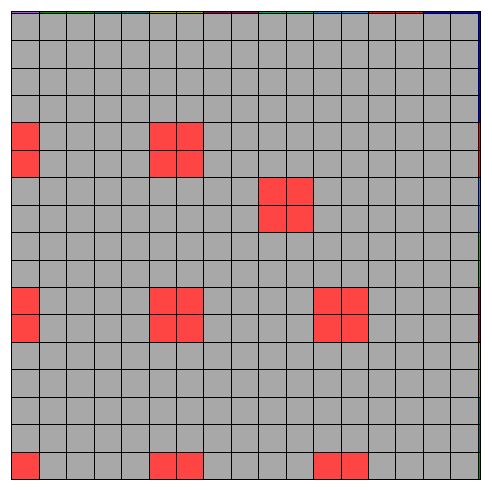
\includegraphics[width=4in]{problem3_radial_mat.png}
  \end{center}
  \caption{\textbf{Fuel assembly mesh and geometry cross section.}
    \textit{Reflecting boundaries are used on the left and lower
      boundaries to create a complete $17 \times 17$ assembly
      geometry. Gray regions are homogenized fuel and red regions are
      homogenized moderator. Each fuel pin is resolved by a $2 \times
      2$ mesh.}}
  \label{fig:problem3_radial_mat}
\end{figure}
\begin{figure}[t!]
  \begin{center}
    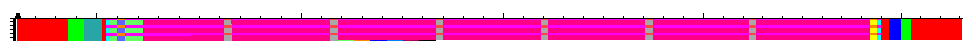
\includegraphics[width=6.0in]{problem3_axial_mat.png}
  \end{center}
  \caption{\textbf{Fuel assembly geometry cross section.} \textit{The
      geometry is subdivided along the axial direction into 50 zones
      spaced to capture material boundaries. Important details include
      spacer grids along the length of the fuel pins and reactor core
      structures on the top and bottom of the assembly. Lighter purple
      material in the center of the assembly is moderator and darker
      purple/red material is fuel.}}
  \label{fig:problem3_axial_mat}
\end{figure}
\begin{figure}[t!]
  \begin{center}
    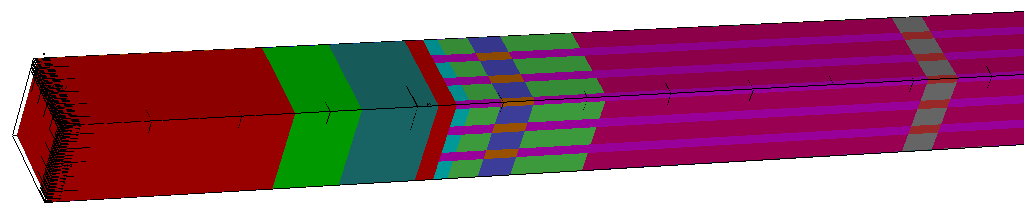
\includegraphics[width=6.0in]{problem3_end.png}
  \end{center}
  \caption{\textbf{Fuel assembly geometry end detail.}
    \textit{Reactor core structure including spacer grids and plenum
      has been included. Lighter purple material on the right of the
      figure is moderator and darker purple/red material is fuel.}}
  \label{fig:problem3_end}
\end{figure}

Significant geometric details are contained in the model including
spacer grids, fuel pins with homogenized cladding and gas gap, core
plenum, and moderator with boron. Group cross sections and other
discrete nuclear data are generated as needed by a cross-section
processing module dependent on the meshing parameters used to
discretize the geometry and single-dimension pin-cell calculations for
initial flux spectrum generation. Table~\ref{tab:problem3_parameters}
gives the primary design parameters for the fuel assembly
calculations.
\begin{table}[h!]
  \begin{center}
    \begin{tabular}{ll}\hline\hline
      \multicolumn{1}{l}{\textbf{Parameter}} & 
      \multicolumn{1}{l}{\textbf{Value}} \\
      Power Level & 0 MW \\
      Inlet Temperature & 326.85C \\
      Fuel Temperature & 600C \\
      Boron Concentration & 1300 ppm \\
      Moderator Density & 0.743 g/cc \\
      Helium Density & \sn{1.79}{-4} g/cc \\
      Zirconium Density & 6.56 g/cc \\
      Stainless Steel Density & 8.0 g/cc \\
      Inconel Density & 8.19 g/cc \\
      UO2 Density & 10.257 g/cc \\
      Fuel Pin Radius (w/o clad) & 0.4096 cm \\
      %%
      \hline\hline
    \end{tabular}
  \end{center}
  \caption{\textbf{Design parameters for the $17 \times 17$ pin fuel
      assembly criticality calculation.}}
  \label{tab:problem3_parameters}
\end{table}

%%---------------------------------------------------------------------------%%
\section{Results}
In this section we present solutions to the fuel assembly problem
using MCSA preconditioning strategies.

\subsection{Block Jacobi Preconditioned Results}
\label{subsec:jacobi_prec_assembly_calc}
Previous work in applying MCSA to the thermal radiation diffusion
equation had success in using Jacobi preconditioning
\cite{evans_monte_2012} and therefore we apply it here to the $SP_N$
equations given their similar diffusion-like form. A single energy
group problem was first computed with $SP_1$ discretization,
effectively giving the one-speed neutron diffusion system for the fuel
assembly resulting in 20,088 degrees of freedom in the
problem. Figure~\ref{fig:block_jacobi_res_mcsa} gives the residual
infinity norm as a function of iteration for the MCSA linear solve in
the first eigenvalue iteration using 25,000 stochastic histories at
every iteration for the adjoint Neumann-Ulam solve.

\begin{figure}[t!]
  \begin{center}
    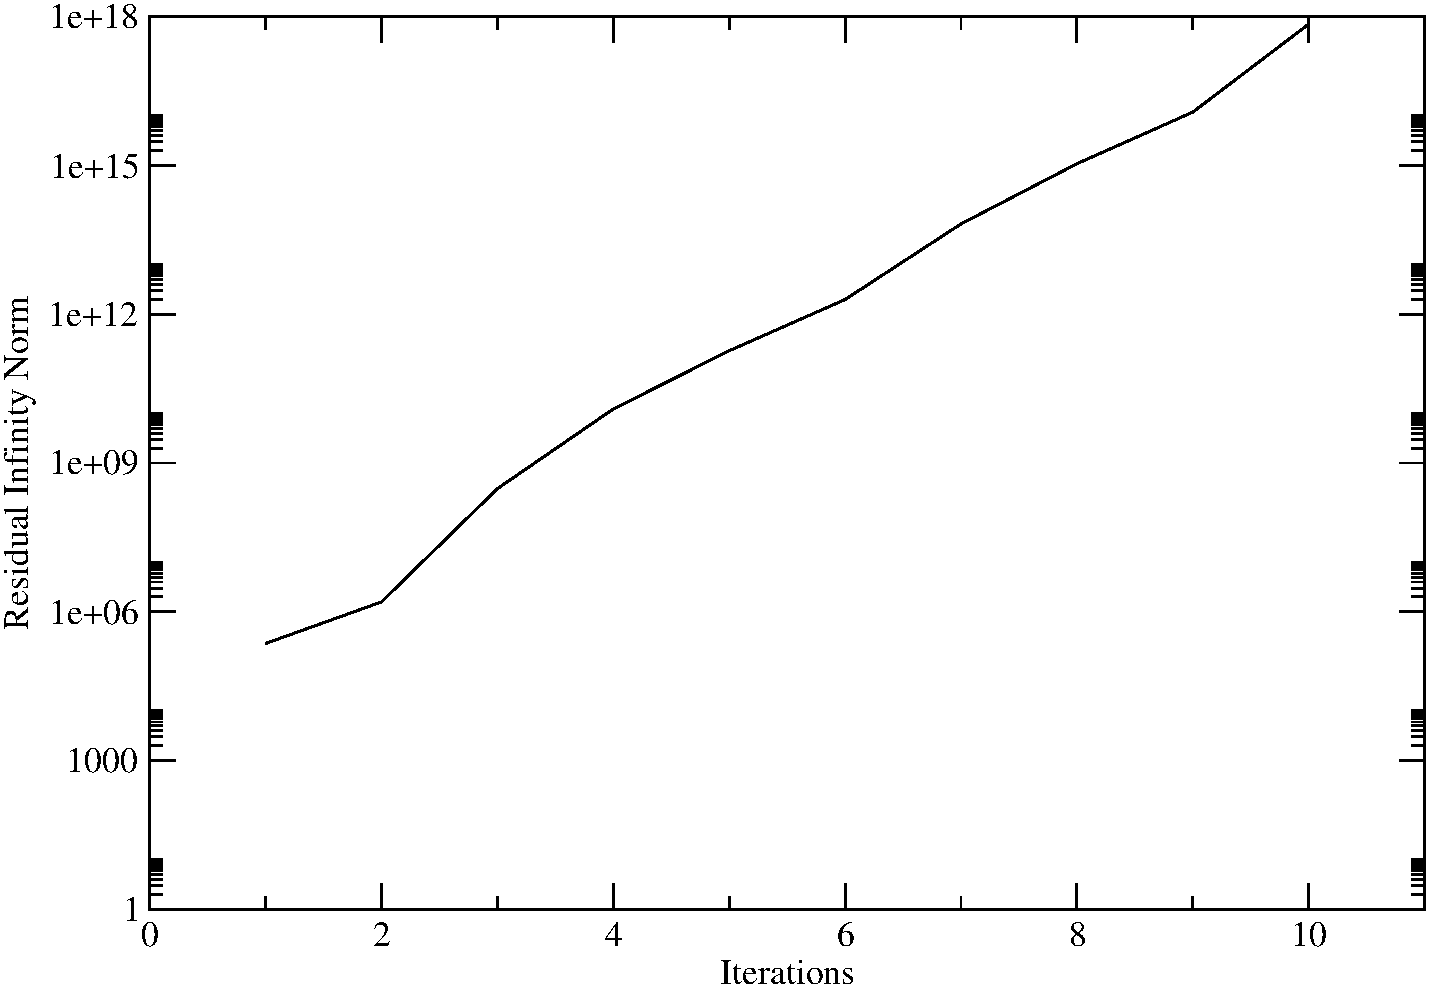
\includegraphics[width=5in]{block_jacobi_res.pdf}
  \end{center}
  \caption{\textbf{Residual infinity norm vs. iteration for the block
      Jacobi preconditioned MCSA solve during the first eigenvalue
      iteration of the 1-group $17 \times 17$ fuel assembly problem.}
    \textit{Convergence was not achieved with the block Jacobi
      preconditioned method.}}
  \label{fig:block_jacobi_res_mcsa}
\end{figure}

Convergence was not achieved as noted by the rapid rise in the
residual over a few iterations. Additional computations performed with
\sn{1}{6} histories per iteration exhibited the same divergent
behavior at a significant computational cost and compute time. To
investigate further, a block Jacobi preconditioned Richardson
iteration was used to solve the same problem. Poor convergence was
observed for the Richardson iteration, however, convergence was
achieved meaning that the preliminary eigenvalue criteria needed to
satisfy MCSA convergence has also been met. With 7291 iterations
required to converge to a tolerance of $\sn{1}{-6}$, $\rho(\mathbf{H})
\approx 0.998$, nearing the limits of MCSA applicability. Based on
these results, it then appears that even if the simple criteria of a
spectral radius of less than one is met and the Richardson iteration
will converge with the same preconditioning, MCSA still may not
converge.

\subsubsection{MCSA Breakdown}
\label{subsubsec:mcsa_break_down}
To study the breakdown of MCSA at iteration matrix spectral radii near
one, we will use the simpler homogeneous 2-dimensional one-speed
neutron diffusion system in a rectilinear grid with vaccuum boundary
conditions to isolate this behavior. In this system, we can vary the
cross sections while maintaining a fixed grid in order to achieve
varying spectral radii. For these studies, we neglect fission as MCSA
behavior is dictated by the transport operator $\mathbf{M}$ in an
eigenvalue scheme with the fission matrix used to generate a fixed
source.

For each solver and estimator combination, the spectral radius of the
iteration matrix generated by the diffusion problem was varied by
changing the absorption cross section from 0.25 to 100 while fixing
the grid size at $100 \times 100$ with $h = 0.1$ and a fixed
scattering cross section of unity. For each parameter variation, a
minimum of one stochastic history per degree of freedom (DOF) in the
problem was used to compute the Monte Carlo correction. If the solver
could not converge in less than 100 iterations, the number of
histories was increased by increments of 5,000 until convergence was
achieved in less than 100 iterations. The number of iterations
required to converge MCSA and the time to converge was recorded as a
means to capture the breakdown.

Figure~\ref{fig:breakdown_iterations} gives the number of iterations
required to converge for the chosen number of histories per iteration
given by Figure~\ref{fig:breakdown_histories} using the adjoint solver
with the collision and expected value estimators and the forward
solver with the collision estimator. For spectral radii less than
0.97, all MCSA problems converged with 1 history per DOF (10,000 total
histories for this problem) with the number of iterations required to
converge increasing as a function of spectral radius. Near a spectral
radius of 0.97, the number of histories required to converge MCSA in
less than 100 iterations takes a dramatic rise that exhibits neither
exponential nor power law behavior. As the spectral radius approaches
1, the number of histories required becomes significant and
effectively impractical to compute. Even with this simple diffusion
problem, the behavior is consistent with that observed for the fuel
assembly problem with $SP_1$ discretization. In that case, we
estimated a spectral radius of $\approx 0.998$, larger than any of the
spectral radii that could be computed within even 90 minutes of
compute time for this simple two dimensional problem. For that large
of a spectral radius, even 1,000,000 histories ($\approx 50$ per DOF)
was not enough to provide convergence. Even if single solve times of
an hour can be tolerated, dozens of solves are typically required to
compute the multiplication factor and flux spectrum within the $SP_N$
eigenvalue scheme for more difficult problems like the fuel assembly,
making the method unusable.
\begin{figure}[t!]
  \begin{center}
    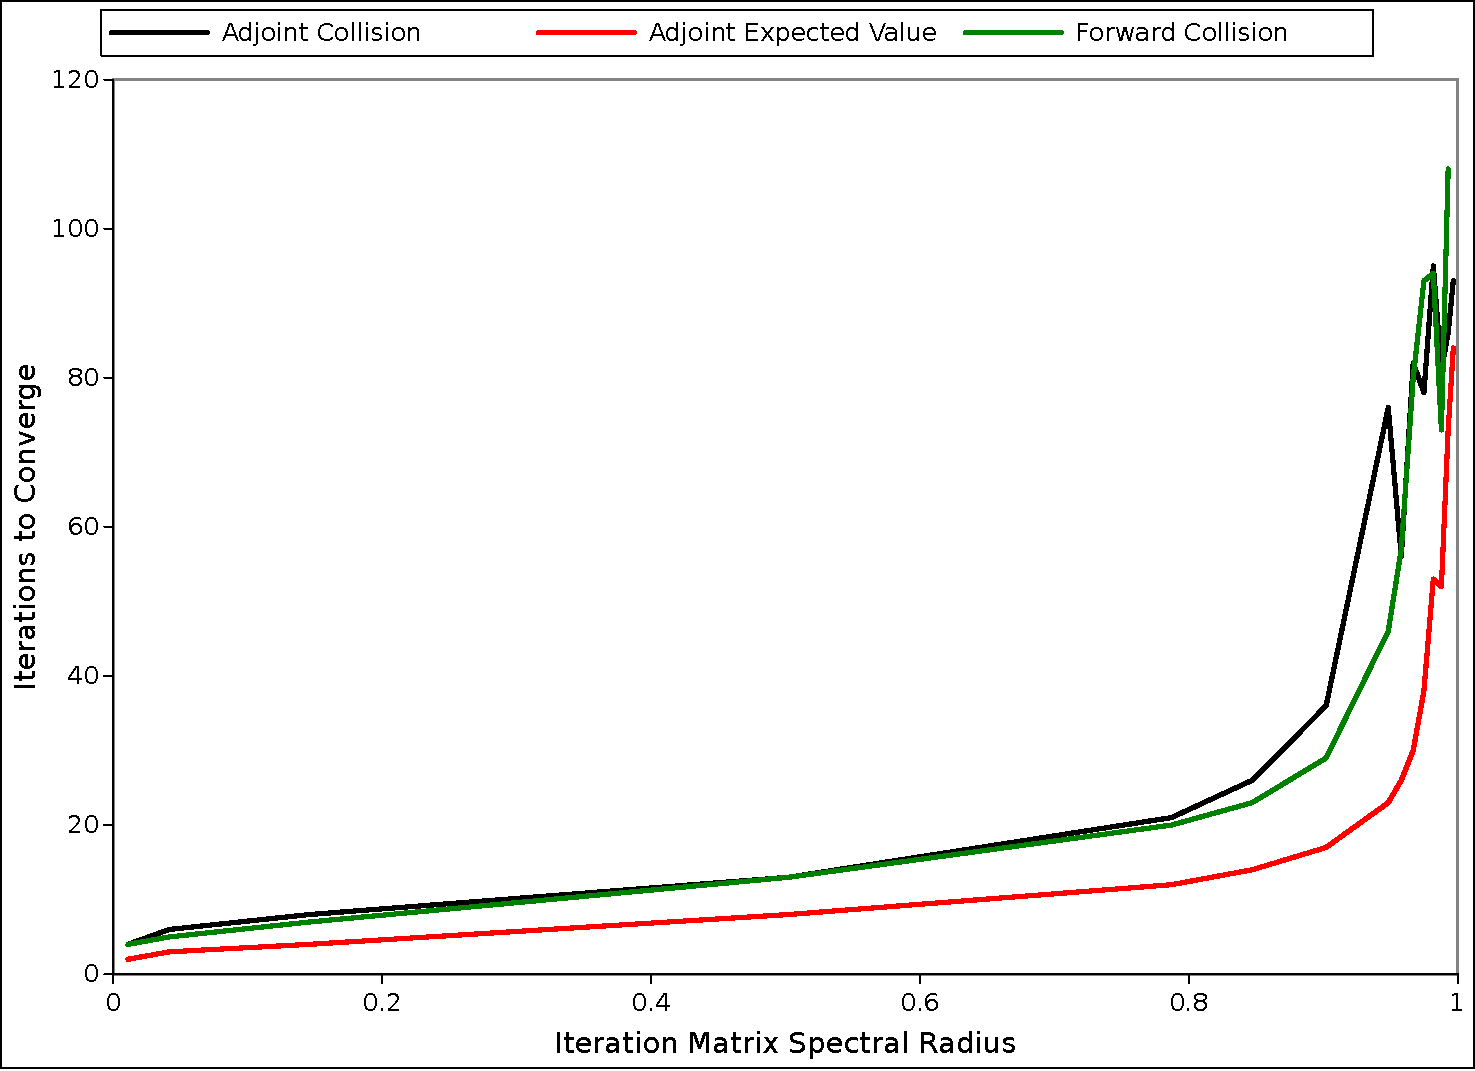
\includegraphics[width=3.5in]{breakdown_iterations.pdf}
  \end{center}
  \caption{\textbf{Iterations required to converge as a function of
      spectral radius for the neutron diffusion problem.} \textit{The
      number of histories was increased to achieve convergence in less
      than 100 iterations. At least 10,000 histories were used for
      each calculation.}}
  \label{fig:breakdown_iterations}
\end{figure}
\begin{figure}[t!]
  \begin{center}
    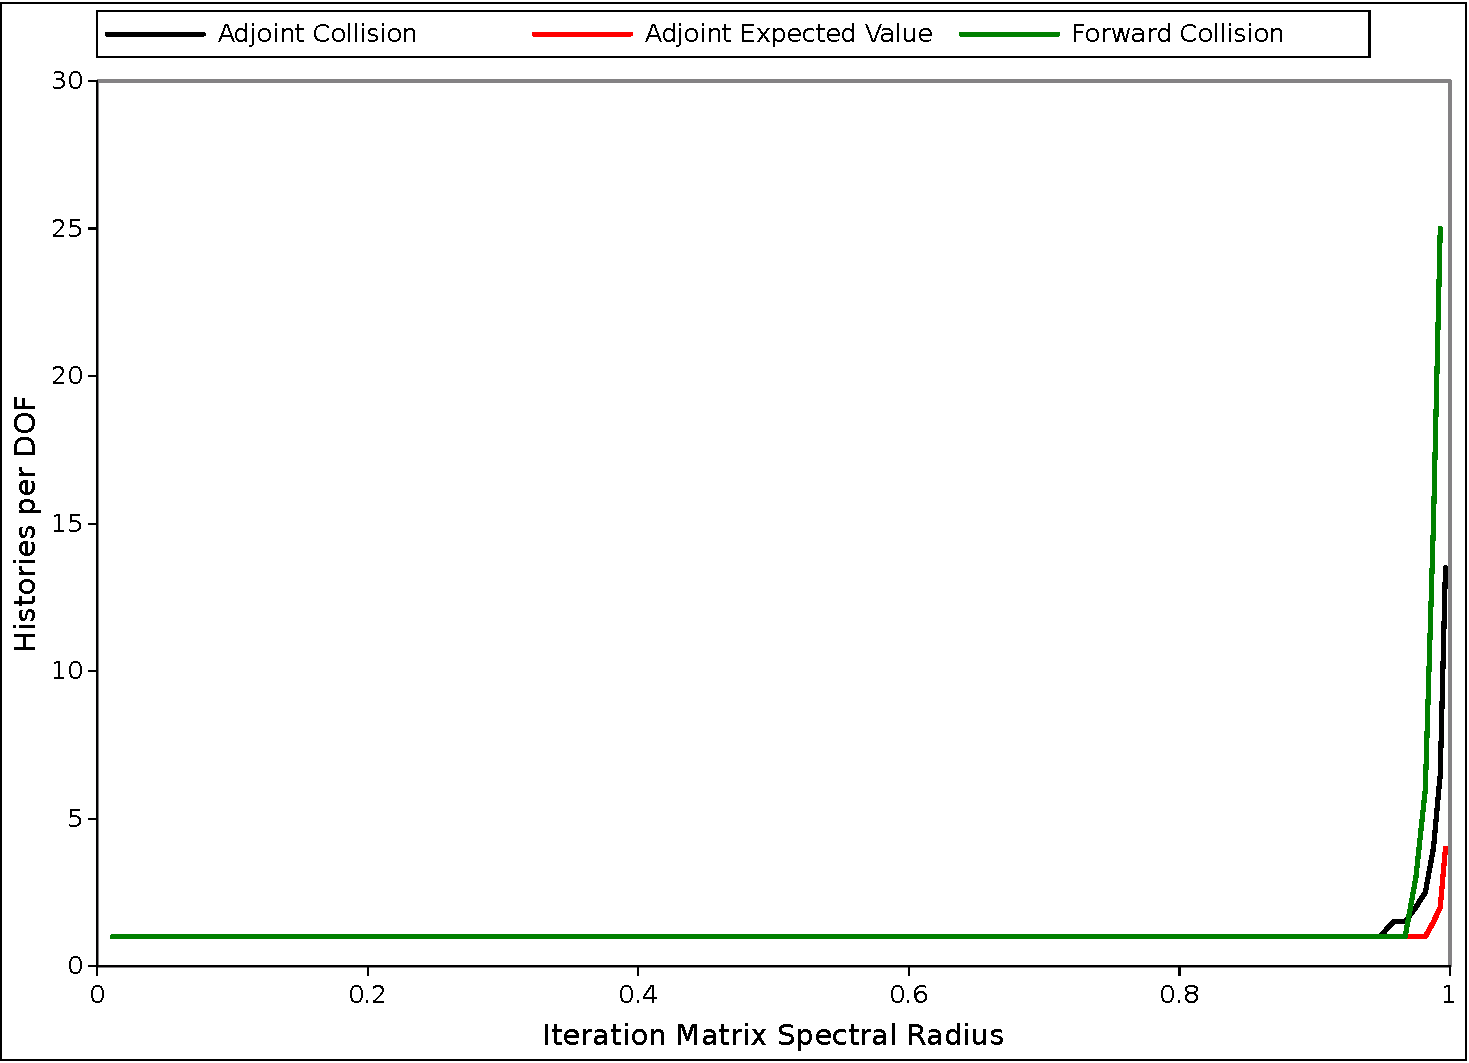
\includegraphics[width=3.5in]{breakdown_histories.pdf}
  \end{center}
  \caption{\textbf{Histories per DOF required to converge as a
      function of spectral radius for the neutron diffusion problem.}
    \textit{The number of histories was increased to achieve
      convergence in less than 100 iterations. At least 10,000
      histories were used for each calculation with 10,000 DOFs in the
      problem.}}
  \label{fig:breakdown_histories}
\end{figure}

In addition to the significantly larger number of histories required
to achieve convergence for ill-conditioned problems another penalty is
paid due to histories that take longer to
compute. Figure~\ref{fig:breakdown_time} gives the CPU time in seconds
required to compute a single random walk averaged over the entire set
of histories run in the calculation over all iterations. As the
spectral radius increases (correlating to a higher ratio of scattering
in the system) the random walk lengths increase, using more CPU time
to finish the computation. Compared to spectral radii of 0.5, larger
spectral radii over 0.97 have histories that require two orders of
magnitude more computation time. This significant increase in
computation time per history coupled with the significant increase in
the number of histories required to converge is evidence that for
problems with spectral radii above $\approx 0.97$, using MCSA to solve
any problems of interest is entirely ineffective and not practical. At
iteration matrix spectral radii this large, using significant numbers
of stochastic histories in the Monte Carlo solve is not enough to
reduce the stochastic uncertainty in the correction, causing the MCSA
sequence to diverge instead of accelerating convergence. We therefore
require a more expansive set of preconditioning techniques to move the
eigenvalue spectrum of the $SP_N$ problem into a regime in which MCSA
is more applicable and in which performance is improved.

\begin{figure}[t!]
  \begin{center}
    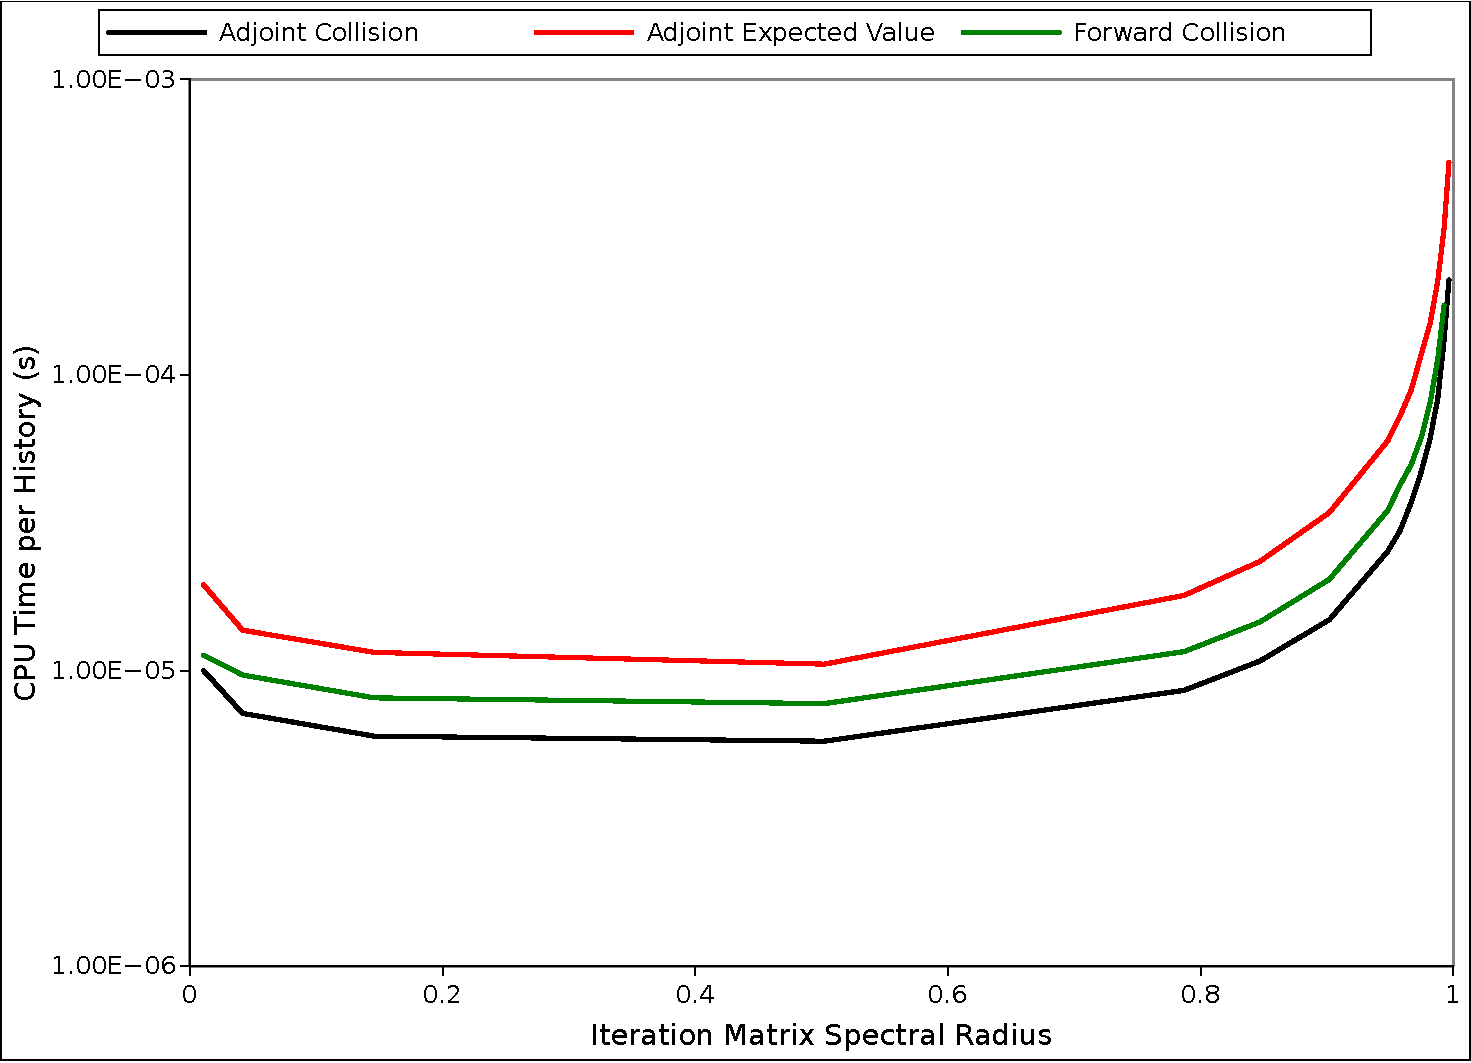
\includegraphics[width=3.5in]{breakdown_time.pdf}
  \end{center}
  \caption{\textbf{CPU time per history as a function of spectral
      radius for the neutron diffusion problem.} \textit{As the
      spectral radius grows, so do the length of the random
      walks. Longer random walks require more CPU time to compute.}}
  \label{fig:breakdown_time}
\end{figure}

\subsection{ILUT Preconditioned Results}
\label{subsec:spn_comparison}
MCSA will now be compared to the same Krylov solvers in terms of both
iterative performance and CPU timing. A Richardson iteration solution
will also be used in order to assess the acceleration provided by the
residual Monte Carlo component of MCSA.  To compare iterative
performance, the number of linear solver iterations required to
converge each eigenvalue iteration was recorded and then averaged over
all eigenvalue iterations for each solver. MCSA solutions to the fuel
assembly problem with 1, 2, and 4 energy groups using $SP_1$
discretization will computed using both BiCGStab and GMRES
implementations from the Trilinos scientific computing library Aztec
\cite{heroux_overview_2005}.

All solvers will be preconditioned with ILUT using a drop tolerance of
\sn{1}{-5} and a fill level of 5. For GMRES, no restrictions were
placed on the size of the subspace and therefore no restarts
occurred. When the collision estimator was used with MCSA, \sn{2}{4}
stochastic histories were used to compute the correction for every
energy group in the problem (\sn{4}{4} and \sn{8}{4} histories total
for the 2 and 4 group calculations respectively) corresponding to
approximately 1 stochastic history per DOF. When the expected value
estimator was used, \sn{5}{2} stochastic histories used for each
energy group (\sn{1}{3} and \sn{1.5}{3} histories total for the 2 and
4 group calculations) giving approximately 1 stochastic history for
every 5 DOFs. The reduced domain approximation was also applied in
conjunction with the ILUT preconditioning using a fill level of 100
and a threshold value of \sn{1}{-10} to reduce the density of states
in the Monte Carlo problem. For relaxation parameters, all MCSA
computations used a Neumann relaxation parameter of 0.7 while a
Richardson relaxation of 1.1 was used with the collision estimator and
1.0 with the expected value estimator. When the collision estimator
was used, an artificial absorption value of 0.2 as outlined in
Appendix~\ref{chap:artificial_absorption} was also
applied. Additionally, both the Richardson-based MCSA iteration given
by Eq~(\ref{eq:mcsa}) and the minimal residual-based MCSA iteration
given by Eq~(\ref{eq:mcsa_min_res}) will be used. A supplementary
performance analysis for this set of MCSA variations is presented in
Appendix~\ref{chap:spn_estimator_comparison}. Table~\ref{tab:spn_solver_defs}
gives definitions for the solvers used to generate the results in the
remainder of this section and Table~\ref{tab:spn_group_structure}
gives the group structures with lower bounds of each group in eV.

\begin{table}[h!]
  \begin{center}
    \begin{tabular}{ll}\hline\hline
      \multicolumn{1}{l}{\textbf{Name}} & 
      \multicolumn{1}{l}{\textbf{Definition}} \\
      BiCGStab-ILUT & BiCGStab preconditioned with ILUT \\
      GMRES-ILUT & GMRES preconditioned with ILUT \\
      MCSA-ILUT-R-C & MCSA preconditioned with ILUT using Richardson \\ 
                    & fixed point iteration and collision estimator \\
      MCSA-ILUT-MR-C & MCSA preconditioned with ILUT using minimal residual \\
                     & fixed point iteration and collision estimator \\
      MCSA-ILUT-R-EV & MCSA preconditioned with ILUT using Richardson \\
                     & fixed point iteration and expected value estimator \\
      MCSA-ILUT-MR-EV & MCSA preconditioned with ILUT using minimal residual \\
                      & fixed point iteration and expected value estimator \\
      Richardson-ILUT & Richardson iteration preconditioned with ILUT \\
      %%
      \hline\hline
    \end{tabular}
  \end{center}
  \caption{\textbf{Solver definitions used for MCSA verification and
      performance analysis.} \textit{The ILUT preconditioner
      parameters were identical for all calculations and solvers.}}
  \label{tab:spn_solver_defs}
\end{table}

\begin{table}[h!]
  \begin{center}
    \begin{tabular}{cl}\hline\hline
      \multicolumn{1}{c}{\textbf{Number of Groups}} & 
      \multicolumn{1}{l}{\textbf{Lower Bounds (eV)}} \\
      1 & \{ \sn{1}{-5} \} \\
      2 & \{ \sn{1}{-1}, \sn{1}{-5} \} \\
      4 & \{ \sn{1}{1}, \sn{1}{0}, \sn{1}{-1}, \sn{1}{-5} \} \\
      %%
      \hline\hline
    \end{tabular}
  \end{center}
  \caption{\textbf{Energy group lower bounds for the multigroup fuel
      assembly criticality problem in electron volts.} \textit{An
      implicit upper bound of \sn{2}{6} eV is assumed for group zero.}}
  \label{tab:spn_group_structure}
\end{table}

For every combination of energy group structure and solver, the
eigenvalue problem was converged with an eigensolver tolerance of
\sn{1}{-6} and a linear solver tolerance of \sn{1}{-8} in a serial
calculation. Table~\ref{tab:serial_ev_results} gives the eigenvalue
computed by each solver for each problem as well as the number of
eigenvalue iterations required to converge. For every problem, each
solver converged to the same eigenvalue up to the number of digits
reported by the eigensolver in the same number of eigenvalue
iterations.

Table~\ref{tab:spn_comparison_iterations} gives this average number of
linear solver iterations required to converge a single eigenvalue
iteration of the fuel assembly problem as a function of the number of
energy groups. In general, the iterative performance of all the
solvers tested aside from the Richardson iteration is comparable with
BiCGStab performing the best. We expect this because not only are the
multigroup $SP_N$ equations positive-definite, but they are also
block-symmetric and therefore we expect the conjugate gradient-based
methods to perform well due to the structure of the projection
scheme. It is important to note that the iterative performance of each
solver is not a strong function of the number of energy groups in the
problem (and therefore the problem size). Even more important,
although BiCGStab produced the best iterative results, MCSA did
perform better than GMRES in many cases with the Richardson iteration
clearly accelerated by the Monte Carlo solve. When compared to the
preconditioned Richardson iteration, the acceleration provided by MCSA
is clear with 3-4 times fewer iterations required for convergence.

It is also important to note the reduced domain approximation
parameters, particularly the fill level, were fixed as the number of
energy groups was increased. By fixing the fill level, we are
effectively fixing the amount of information contained in the
composite linear operator available for the Monte Carlo
problem. Limiting this information to 100 entries per row in the
preconditioned system did not appear to have a significant effect on
the iterative performance of the solver. For larger numbers of energy
groups (and therefore DOFs) this may be an issue and this number may
need to be increased to maintain iterative performance. Currently,
memory restrictions arising from the explicit preconditioning strategy
prevent larger numbers of energy groups to be analyzed using an
appropriate preconditioner for the fuel assembly problem.

\begin{table}[h!]
  \begin{center}
    \begin{tabular}{lccc}\hline\hline
      \multicolumn{1}{l}{Solver}&
      \multicolumn{1}{c}{1 Group}&
      \multicolumn{1}{c}{2 Groups}&
      \multicolumn{1}{c}{4 Groups}\\
      \hline
      BiCGStab-ILUT & 11.6 & 11.6 & 12.4 \\ 
      GMRES-ILUT & 18.1 & 17.9 & 18.9 \\
      MCSA-ILUT-R-C & 14.6 & 15.4 & 17.6 \\
      MCSA-ILUT-MR-C & 16.0 & 17.1 & 23.7 \\
      MCSA-ILUT-R-EV & 18.3 & 19.4 & 16.8 \\
      MCSA-ILUT-MR-EV & 19.6 & 22.4 & 17.5 \\
      Richardson-ILUT & 60.9 & 60.4 & 63.4 \\
      %%
      \hline\hline
    \end{tabular}
  \end{center}
  \caption{\textbf{Average number of linear solver iterations
      iterations required to converge the fixed source $SP_N$ problem
      at each eigenvalue iteration for the fuel assembly problem for
      1, 2 and 4 energy groups.} \textit{Values are rounded to the
      first decimal place. Table~\ref{tab:spn_solver_defs} gives the
      description for each solver type presented.}}
  \label{tab:spn_comparison_iterations}
\end{table}

Although iterative performance for MCSA was comparable to that
observed for Krylov implementations using exactly the same
preconditioning scheme, timing performance is not as
competitive. Figure~\ref{fig:spn_comparison_time} gives the average
CPU time per linear solver iteration required to converge the fuel
assembly problem with all linear solver iterations over all eigenvalue
iterations used to compute the average. The Krylov solver
implementations are approximately an order of magnitude faster than
the MCSA implementations presented here. We expect these results for
several reasons. First, even when the reduced domain approximation is
used there are $O(100)$ elements in each row of the system and each of
those elements must be accessed for next-event sampling and tally
vector modification during a transition in the Monte Carlo random walk
sequence. In addition, although the preconditioned fixed point
iterations used in the MCSA sequence do not use the composite linear
operator but rather a sequence of matrix vector multiplies to achieve
the same preconditioning effect, they do use the explicitly extracted
inverse of the preconditioning matrices which themselves are dense,
leading to exceedingly slow computation times even in the fixed point
iteration.

From a timing perspective, the greatest burden is the time required to
actually form the explicit inverse preconditioner matrices and the
composite operator through matrix-matrix multiplication. The timing
numbers reported were simply to perform the MCSA iteration procedure
with the composite operator already
formed. Figure~\ref{fig:spn_comparison_time} additionally presents the
CPU times for MCSA convergence with the time to form the inverse of
the preconditioners and the composite linear operator through
matrix-matrix multiplication amortized over all iterations. As is
readily observed, including the costs of these operations increases
the MCSA computation time by another order of magnitude.

\begin{figure}[t!]
  \begin{center}
    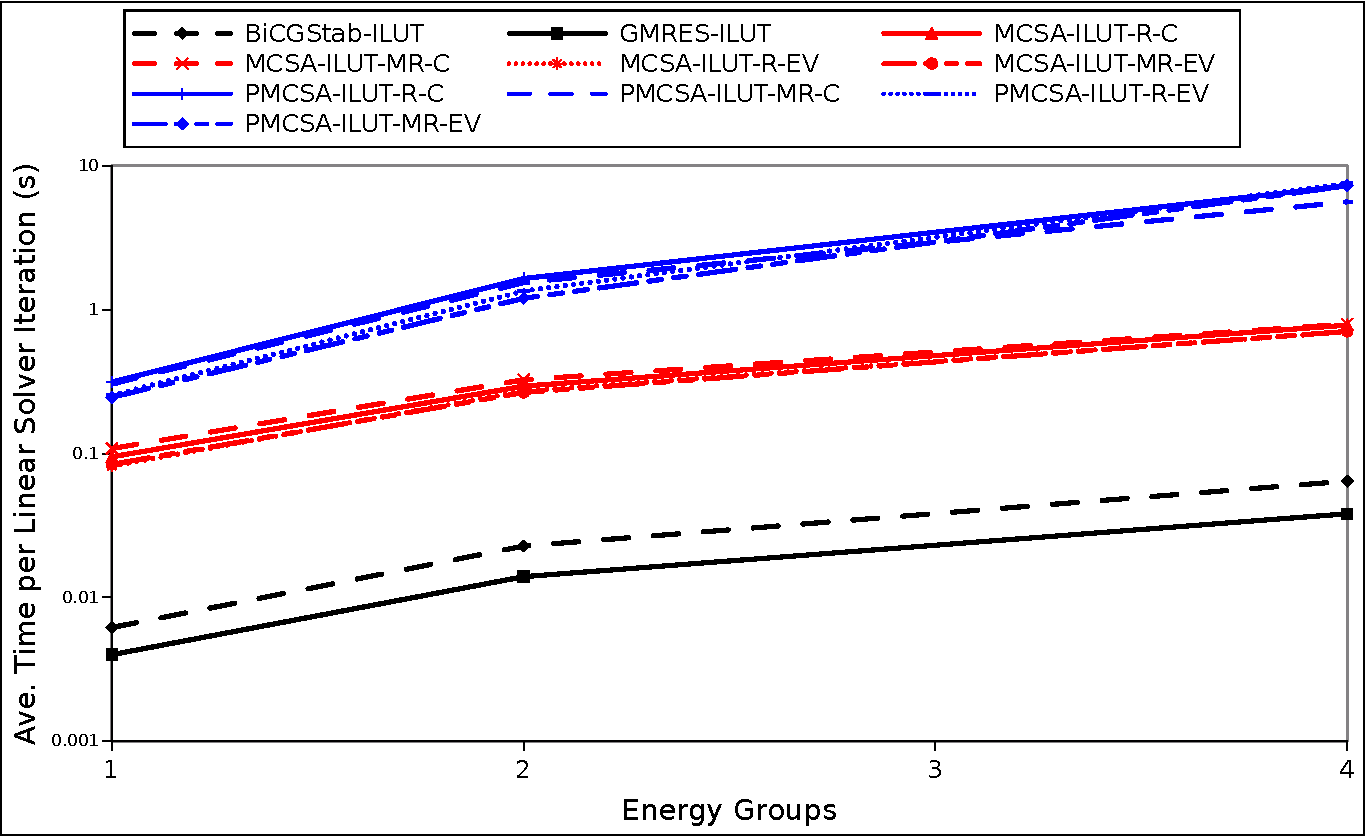
\includegraphics[width=5in]{solver_p_time.pdf}
  \end{center}
  \caption{\textbf{Average CPU time per iteration in seconds for the
      fuel assembly problem as a function of energy groups with
      preconditioning time included for the MCSA methods.}
    \textit{All linear solver iterations over all eigenvalue
      iterations were used to compute the
      average. Table~\ref{tab:spn_solver_defs} gives the description
      for each solver type presented in the legend. Data labeled
      starting with PMCSA and shown in blue is identical to those
      labeled with MCSA except that they additionally include the cost
      of generating the inverse of the preconditioners and composite
      linear operator.}}
  \label{fig:spn_comparison_time}
\end{figure}

For the Krylov methods, the ILUT preconditioners are applied to a
vector with two triangular solves, one for each triangular
factor. Also, the original linear operator has $O(10)$ elements in
each row of the system, an order of magnitude less than that used in
the reduced domain composite operator. Second, the implementation
presented here has not been optimized and it is likely that several
components of the algorithm can be implemented in a more desirable
time complexity. However, it is most important to note here that the
CPU timing data presented in Figure~\ref{fig:spn_comparison_time}
shows that all methods have the same time complexity; their
differences are merely the manifestation of a large time constant due
to the effects of the explicit preconditioning scheme. For transport
systems where this is not a problem, the literature explicitly shows
that MCSA can be competitive with these production Krylov methods
using CPU time as a measure \cite{evans_monte_2012}.

Based on the performance results in this section, MCSA shows promise
as a competitive method for solutions to the neutron transport problem
discretized with the $SP_N$ approximation and could potentially be
superior if the preconditioning strategy were improved to reduce time
to solution and memory usage. Not only are the correct answers
produced when compared to production linear solvers, but the iterative
performance is comparable to Krylov methods with identical
preconditioning that would typically be used most calculations. From a
CPU timing perspective, the methods yield the same time complexity as
a function of the number of energy groups in the problem when compared
to the Krylov methods. Here, a large time constant is generated due to
the explicit preconditioning strategy and the generation of dense
linear operators as a result. To improve these results and put general
MCSA schemes into a performance regime where they are competitive with
Krylov methods for neutron transport problems, significant research
will be required to improve upon the explicit preconditioning scheme
presented here.

%%---------------------------------------------------------------------------%%
\section{Conclusion}
\label{sec:conclusion}

In this paper, the Monte Carlo Synthetic Acceleration method has been
applied to the $SP_N$ discretization of the neutron transport equation
and explored in the context of a difficult nuclear fuel assembly
criticality problem. We observed that MCSA can solve the asymmetric
system generated by the $SP_N$ equations by incorporating the solution
technique into the Exnihilo neutronics code base developed at Oak
Ridge National Laboratory. In contrast to the thermal radiation
diffusion problem addressed in our previous work, light water reactor
problems are difficult to solve with MCSA as they have large spectral
radii due to the neutron scattering in the moderator. Because of this,
simple Jacobi-based preconditioning reduces the spectral radius of the
$SP_N$ system below unity, however, this alone was discovered not to
be sufficient criteria alone for MCSA convergence. As the spectral
radius approaches unity, MCSA was demonstrated to break down with more
stochastic histories required for convergence and more CPU time
required per history. To alleviate these effects, a left-right
preconditioned form of the MCSA method was developed and applied to
the $SP_N$ equations to obtain convergence. For the nuclear fuel
assembly problem, MCSA was observed to converge in fewer iterations
per eigenvalue iteration than GMRES for the fuel assembly criticality
problem and more than Bi-CGStab using the same
preconditioning. However, the explicit preconditioning strategy
required to overcome the MCSA spectral radius restriction creates run
times $O(100)$ larger than the production Krylov methods for the fuel
assembly criticality problem, indicating that significant research in
the area of Monte Carlo preconditioning implementations is required in
order for the method to be competetive in terms of time to solution.

%%---------------------------------------------------------------------------%%
\pagebreak
\bibliographystyle{ieeetr} 
\bibliography{references}
\end{document}


